\documentclass{tarea}

\profesor{Ricardo Muñoz}
\auxiliar{Sebastián Villalón}
\ayudante{Victoria Caballero}
\curso{Meteorología Física}
\ntarea{5}
\author{Benjamín Edwards}
\date{\Mes, \the\year}

\titleformat{\subsection}{\bfseries\large}{Problema \thesubsection}{5mm}{}

\begin{document}

\maketitle

\setcounter{section}{4}
\setcounter{subsection}{13}
\subsection{}
El espectro de densidad de flujo presentado corresponde al que se muestra en la siguiente figura.

\begin{figure}[htpb]
    \centering
    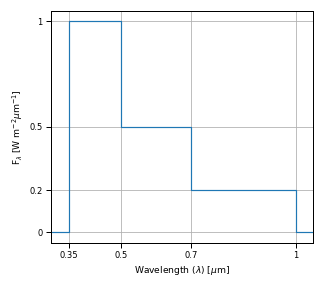
\includegraphics[]{figs/F_lambda}
    \caption{Densidad de flujo monocromática}
    \label{fig:F_lambda}
\end{figure}
Luego, la densidad de flujo total corresponde a la integral de $F_\lambda$ respecto de $\lambda$. Esto resulta la integral o el área bajo la curva de la figura \ref{fig:F_lambda}, lo que en este caso particular resulta un valor de
\begin{equation}
    F = 0.31\text{ W m$^{-2}$} \label{F}
\end{equation}
%%%%%%%%%%%%%%%%%%%%%%%%%%%%%%%%%%%%%%%%%%%%%%%%%%%%%%%%%%
%%%%%%%%%%%%%%%%%%%%%%%%%%%%%%%%%%%%%%%%%%%%%%%%%%%%%%%%%%
%%%%%%%%%%%%%%%%%%%%%%%%%%%%%%%%%%%%%%%%%%%%%%%%%%%%%%%%%%
\subsection{}
Recordemos que la absortividad $\alpha_\lambda$ se define como
\begin{equation}
    \alpha_\lambda = \frac{I_\lambda (\text{absorbida})}{I_\lambda (\text{incidente})} \nonumber
\end{equation}
De acá podemos despejar $I_\lambda (\text{absorbida})$ como
\begin{equation}
    I_\lambda (\text{absorbida}) = \alpha_\lambda I_\lambda (\text{incidente}) \label{Iabs}
\end{equation}
y si integramos podemos obtener la irradiancia (F). Para esto, multiplicamos en ambos lados de \eqref{Iabs} por $\cos\theta$ e integramos con respecto al ángulo sólido
\begin{equation}
    F_\lambda (\text{absorbida}) = \int_\Omega I_\lambda (\text{absorbida}) \cos\theta \, d\Omega = \int_\Omega \alpha_\lambda I_\lambda (\text{incidente}) \cos\theta \, d\Omega \nonumber
\end{equation}
Si consideramos la absortividad como isotrópica, de modo que no dependa de la dirección $(\theta,\phi)$, podemos sacarla de la integral, obteniendo
\begin{equation}
    F_\lambda (\text{absorbida}) = \alpha_\lambda \int_\Omega I_\lambda (\text{incidente}) \cos\theta \, d\Omega  = \alpha_\lambda F_\lambda (\text{incidente}) \nonumber
\end{equation}
Ahora, para calcular toda la densidad de flujo integramos en $\lambda$
 \begin{equation}
    F (\text{absorbida}) = \int_0^{\infty} \alpha_\lambda F_\lambda (\text{incidente}) \, d\lambda \nonumber
\end{equation}
Notemos que $F_\lambda (\text{incidente})$ corresponde al espectro del problema anterior. Considerando también que la absortividad del enunciado es
\begin{equation}
    \alpha_\lambda = \begin{cases}
            0 &\text{ si $\lambda < 0.7\mu$m}\\
            1 &\text{ si $\lambda > 0.7\mu$m}
    \end{cases} \nonumber
\end{equation}
tenemos que $F_\lambda (\text{absorbida})$ es de 0.06 W m$^{-2}$.\\

Para el caso de la radiación reflejada consideraremos que
\begin{equation}
    \alpha_\lambda + R_\lambda + T_\lambda = 1, \label{conservI}
\end{equation}
con $R$ la reflectividad y $T_\lambda$ la transmisividad. Ahora, como la superficie es opaca consideraremos $T_\lambda=0$, obteniendo así
$$R_\lambda = 1 - \alpha_\lambda$$

Siguiendo la misma lógica anterior, la radiación reflejada es
\begin{equation}
   F (\text{reflejada}) = \int_0^{\infty} (1 - \alpha_\lambda) F_\lambda (\text{incidente}) \, d\lambda \nonumber
\end{equation}
lo que corresponde a 0.25 W m$^{-2}$.

%%%%%%%%%%%%%%%%%%%%%%%%%%%%%%%%%%%%%%%%%%%%%%%%%%%%%%%%%%%%%%%%%
%%%%%%%%%%%%%%%%%%%%%%%%%%%%%%%%%%%%%%%%%%%%%%%%%%%%%%%%%%%%%%%%%
%%%%%%%%%%%%%%%%%%%%%%%%%%%%%%%%%%%%%%%%%%%%%%%%%%%%%%%%%%%%%%%%%

\setcounter{subsection}{42}
\subsection{}

Tenemos que la radiancia luego de pasar por una capa corresponde a
\begin{equation}
    I_\lambda (\text{transmitida}) = I_\lambda (\text{incidente}) T_\lambda \nonumber
\end{equation}
donde $T_\lambda$ corresponde a la transmisividad de la capa, definida como
 $$T_\lambda = e^{-\tau_\lambda \sec\theta}$$
con $$\tau_\lambda = \int_{z_1}^{z_2} k_\lambda \rho r \, dz$$
y $\rho$ y $r$ la densidad y razón de mezcla del gas de la capa.\\

Como en el enunciado mencionan que el ángulo zenital es cero, entonces $\sec\theta = 1$. También mencionan que $k_\lambda = 0.01$ m$^{2}$ Kg$^{-1}$. De esto asumimos que $k_\lambda$ es constante en toda la capa, por lo tanto
\begin{equation}
    \tau_\lambda = k_\lambda \int_{z_1}^{z_2} \rho r dz \label{tau1}
\end{equation}
Notamos que la integral en \eqref{tau1} corresponde a la cantidad de masa por unidad de área, valor que también nos informan en el enunciado (1 Kg m$^{-2}$) (también hemos asumido $r=1$, ya que solo nos mencionan la presencia de un solo gas en la capa). Remplazando estos valores, obtenemos que $\tau_\lambda = 0.01$ y luego que $T_\lambda = e^{-0.01}$.\\

Ahora, considerando que no hay reflectividad, de \eqref{conservI} tenemos que la absortividad es
$$\alpha_\lambda = 1 - T_\lambda = 1 - e^{-0.01} \simeq 0.00995$$

Como este valor no depende de $\lambda$ ni de la dirección, podemos asegurar que apenas un $0.995 \%$ de la radiación es absorbida.\\

Ahora determinaremos cuanta masa de este gas se requeriría para absorber la mitad de la radiación. Para esto buscamos que cantidad de masa por unidad de area nos permite obtener $\alpha_\lambda = 1 - T_\lambda = 0.5$, o de otra forma, la solución de $u$ en 
$$ 0.5 = e^{-0.01 u} $$
Despejando $u$ obtenemos
$$u = \dfrac{\ln(0.5)}{-0.01} \text{ Kg m}^{-2},$$
es decir, que se requerirían aproximadamente 69.31 Kg m$^{-2}$.

\setcounter{subsection}{45}
\subsection{}

Usaremos la ecuación hipsométrica en la siguiente forma
\begin{equation}
    p_2 = p_1 \exp \left[\dfrac{-(z_2-z_1)}{H}\right] \nonumber
\end{equation}
con $H = \dfrac{g}{RT}$ la altura de escala.\\

Si consideramos $p_1$ la presión superficial (en $z_{1} = 0$ m), tenemos la siguiente expresión para la presión en función de la altura.
\begin{equation}
    p(z) = p_1 \exp \left[\dfrac{-z}{H}\right] \label{press}
\end{equation}

Ahora, como la temperatura no cambia con la altura (lapse rate isotermal), podemos usar la ecuación de estado 
$$p = \rho RT,$$
en cada instante. Luego, si la remplazamos en \eqref{press}, podemos obtener una expresión para la densidad
\begin{equation}
    \rho(z) = \rho_1 \exp \left[\dfrac{-z}{H}\right] \label{density}
\end{equation}
con $\rho_1$ la densidad al nivel de la superficie.

Por otro lado tenemos, estamos buscando la altura $h$ en la cual el espesor óptico
\begin{equation}
\tau_\lambda = \int_0^{h}  k_\lambda \rho r \, dz, \label{tau}
\end{equation}
es 1.
Consideramos que $k_\lambda$ no cambia con la altura, por lo que lo podemos sacar de la integral. También, como esta atmósfera hipotética es ta completamente formado de este gas, la razón de mezcla $r$ es 1. 
Ahora, remplazaremos la expresión para la densidad \eqref{density} en \eqref{tau}
$$1 = k_\lambda \int_0^{h} \rho_1 \exp \left[\dfrac{-z}{H}\right] \, dz$$
Integramos y obtenemos
$$1 = k_\lambda \rho_1 (-H) \left( e^{-h/H} - 1 \right) $$
Ahora, despejamos $h$.
\begin{equation}
h = -H \ln \left( \frac{k_\lambda \rho_1 H -1}{k_\lambda \rho_1 H} \right) \label{h}
\end{equation}

Dado que sabemos el valor de la altura de escala $H$ (10 Km), y el del coeficiente de absorción másico $k_\lambda$ (0.01 m$^{-2}$ Kg$^{-1}$), para obtener el valor de $h$ solo nos falta obtener la densidad $\rho_1$. Para esto usaremos la definición de la altura de escala $H$, de la cual se desprende que $gH = RT$. Acá usaremos que $g = 10$ m s$ ^{-2}$, entonces $RT = 10^{5}$ m$^{2}$ s$^{-2}$. Ahora, usando la ecuación de estado $p = \rho RT$ al nivel de superficie obtenemos.
\begin{equation}
    \rho_1 = \frac{P_1}{RT}
\end{equation}
Como la presión atmosférica al nivel de superficie es de $10^{5}$ Pa, tenemos que la densidad $\rho_1$ es de 1 Kg m$^{-3}$.\\

Remplazando $\rho_1 = 1$ Kg m$^{-3}$ en la ecuación \eqref{h} obtenemos que esta altura corresponde a $$ h = -10^{4} \ln \left( 99/100 \right) \text{ m} \simeq 100.5 \text{ m} $$
Evaluamos este valor en la ecuación \eqref{press} y obtenemos que la presión en ese punto es de 
$$p_2 = p_1 e^{h/H} = p_1 \cdot 0.99 $$
Considerando que $p_1 = 1000$ hPa, tenemos que la presión al nivel de altura $h$ es de 990 hPa.






\end{document}
